\clearpage
\section{Quantum Random Number Generator}

\begin{tcolorbox}	
\begin{tabular}{p{2.75cm} p{0.2cm} p{10.5cm}} 	
\textbf{Students Name}  &:& Mariana Ramos (12/01/2018 - )\\
\textbf{Goal}          &:& sdf/quantum\_random\_number\_generator.
\end{tabular}
\end{tcolorbox}

True random numbers are indispensable in the field of cryptography to guarantee the security of the communication protocols \cite{katsoprinakis2008quantum}. There are two approaches for random number generation, which in some applications must be unpredictable: the pseudorandom generation which are based on some kind of classical algorithms implemented on a computing device, or the physical random generators which consist in measuring some physical observable with random behaviour.

In this chapter, it is presented the theoretical analysis and simulation of a quantum random generator by measuring the polarization of single photons with a polarizing beam splitter.

\subsection{Theoretical Analysis}

Nowadays, the only known way to generate truly random numbers is by building a physical source by using quantum mechanical decisions, since the occurrence of each individual result of such a quantum mechanical decision is truly random, ie it is inestimable or unknowable \cite{Zeilinger}. One of the optical processes available as a source of randomness is the splitting of a polarized single photon beam.

\begin{figure}[H]
    \centering
        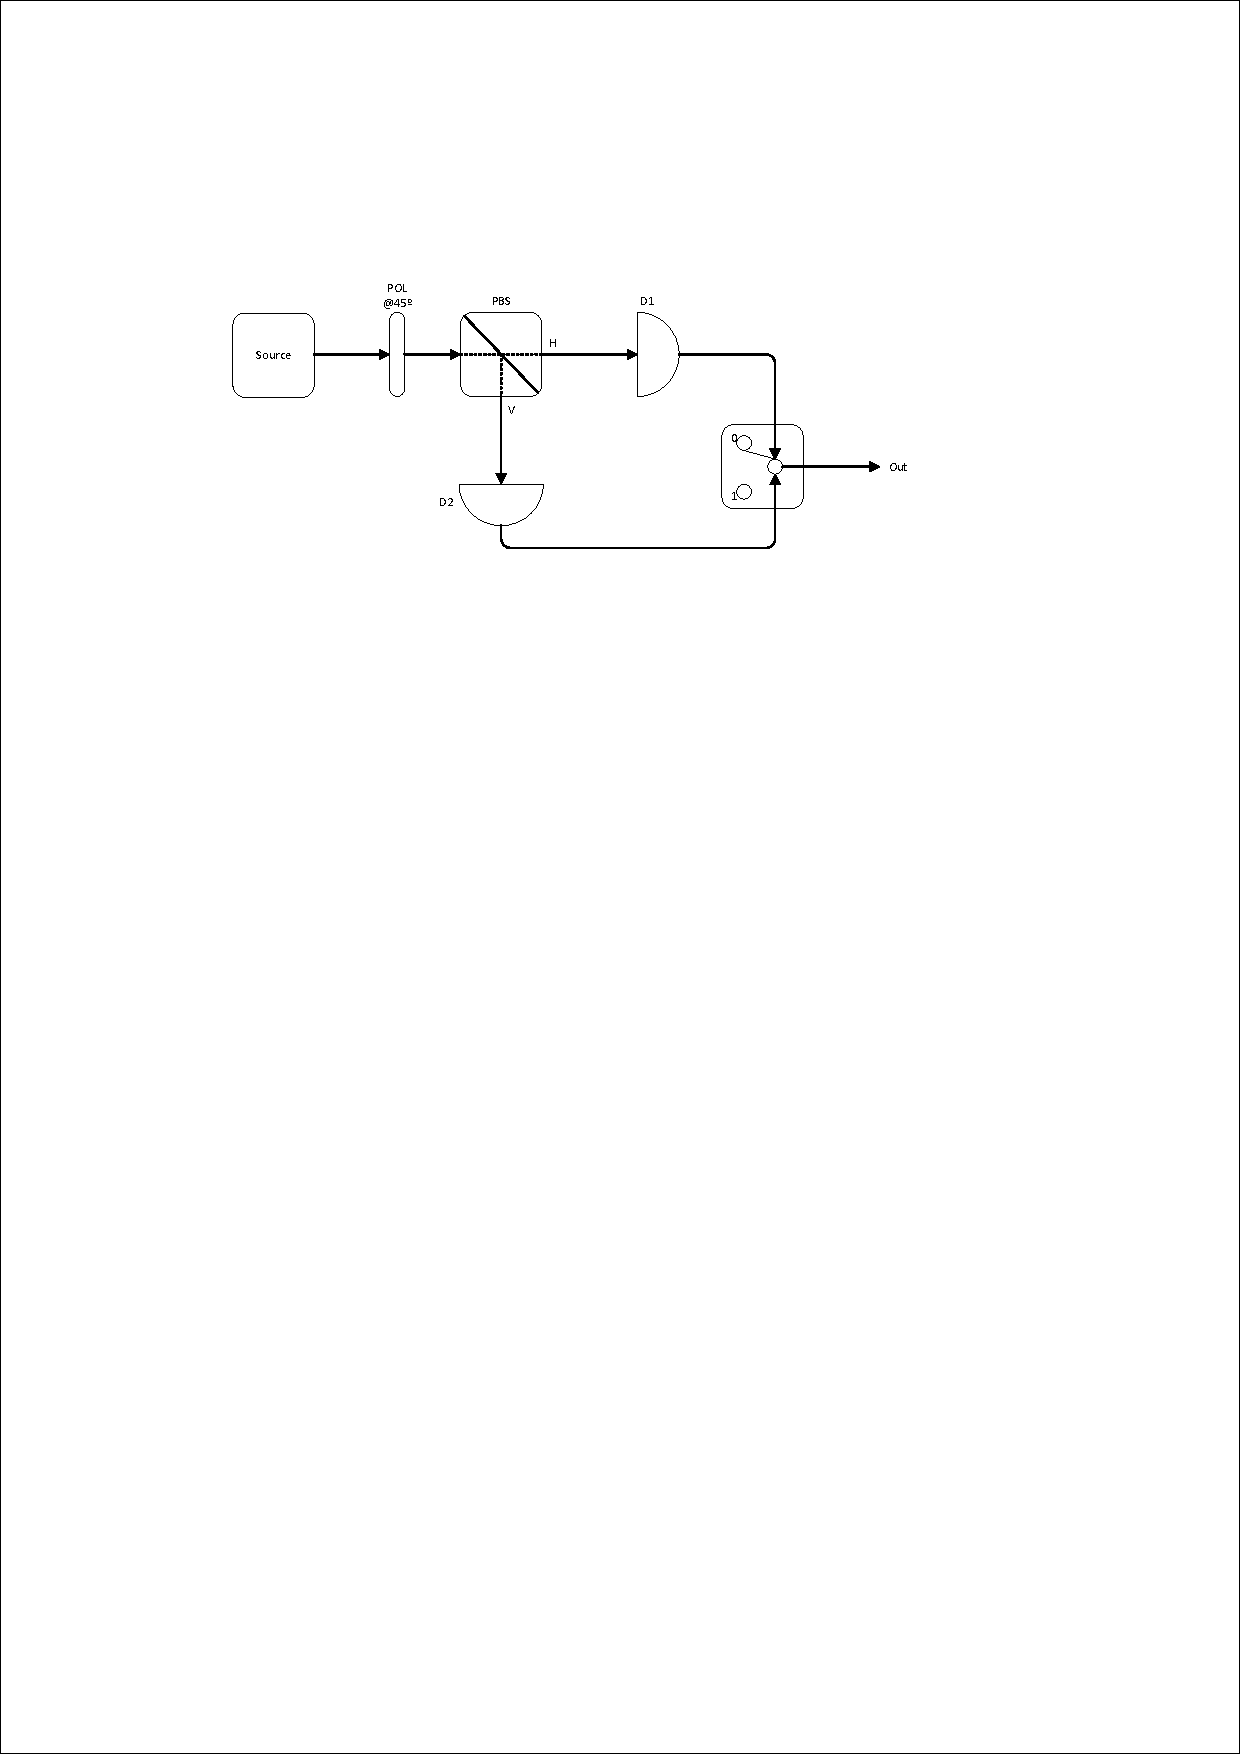
\includegraphics[clip, trim=3cm 20cm 5cm 5cm, width=1.00\textwidth]{./sdf/quantum_random_number_generator/figures_raw/Random_Number_Generator.pdf}
    \caption{Source of randomness with a polarization beam splitter PBS where the incoming light is polarized with POL at $45^{\circ}$ with respect to the PBS. Figure adapted from \cite{Zeilinger}.}\label{qrng}
\end{figure}

The principle of operation of the random generator is shown in figure \ref{qrng}. Each individual photon coming from the source is polarized at $45^\circ$ and has equal probability of found in the horizontal polarization (H) or in the vertical polarization (V) output of the PBS. However, quantum theory estimates for both cases the individual choices are truly random and independent one from each other. This way, the detection of the photons in each output of the polarization beam splitter is done with single photon detectors and combining the detection pulse in a switch, which has two possible states: '0' or '1'. When the detector \textbf{D1} fires, the switch is flipped to state '0' and does not mode until a detection event in detector \textbf{B2} occurs and it does not move until a detection occurs in detector \textbf{D1}. In the case of some detections occur in a row in the same detector, only the first detection clicks and the following detections leave the switch unaltered.

\subsection{Simulation Analysis}

\begin{figure}[h]
    \centering
        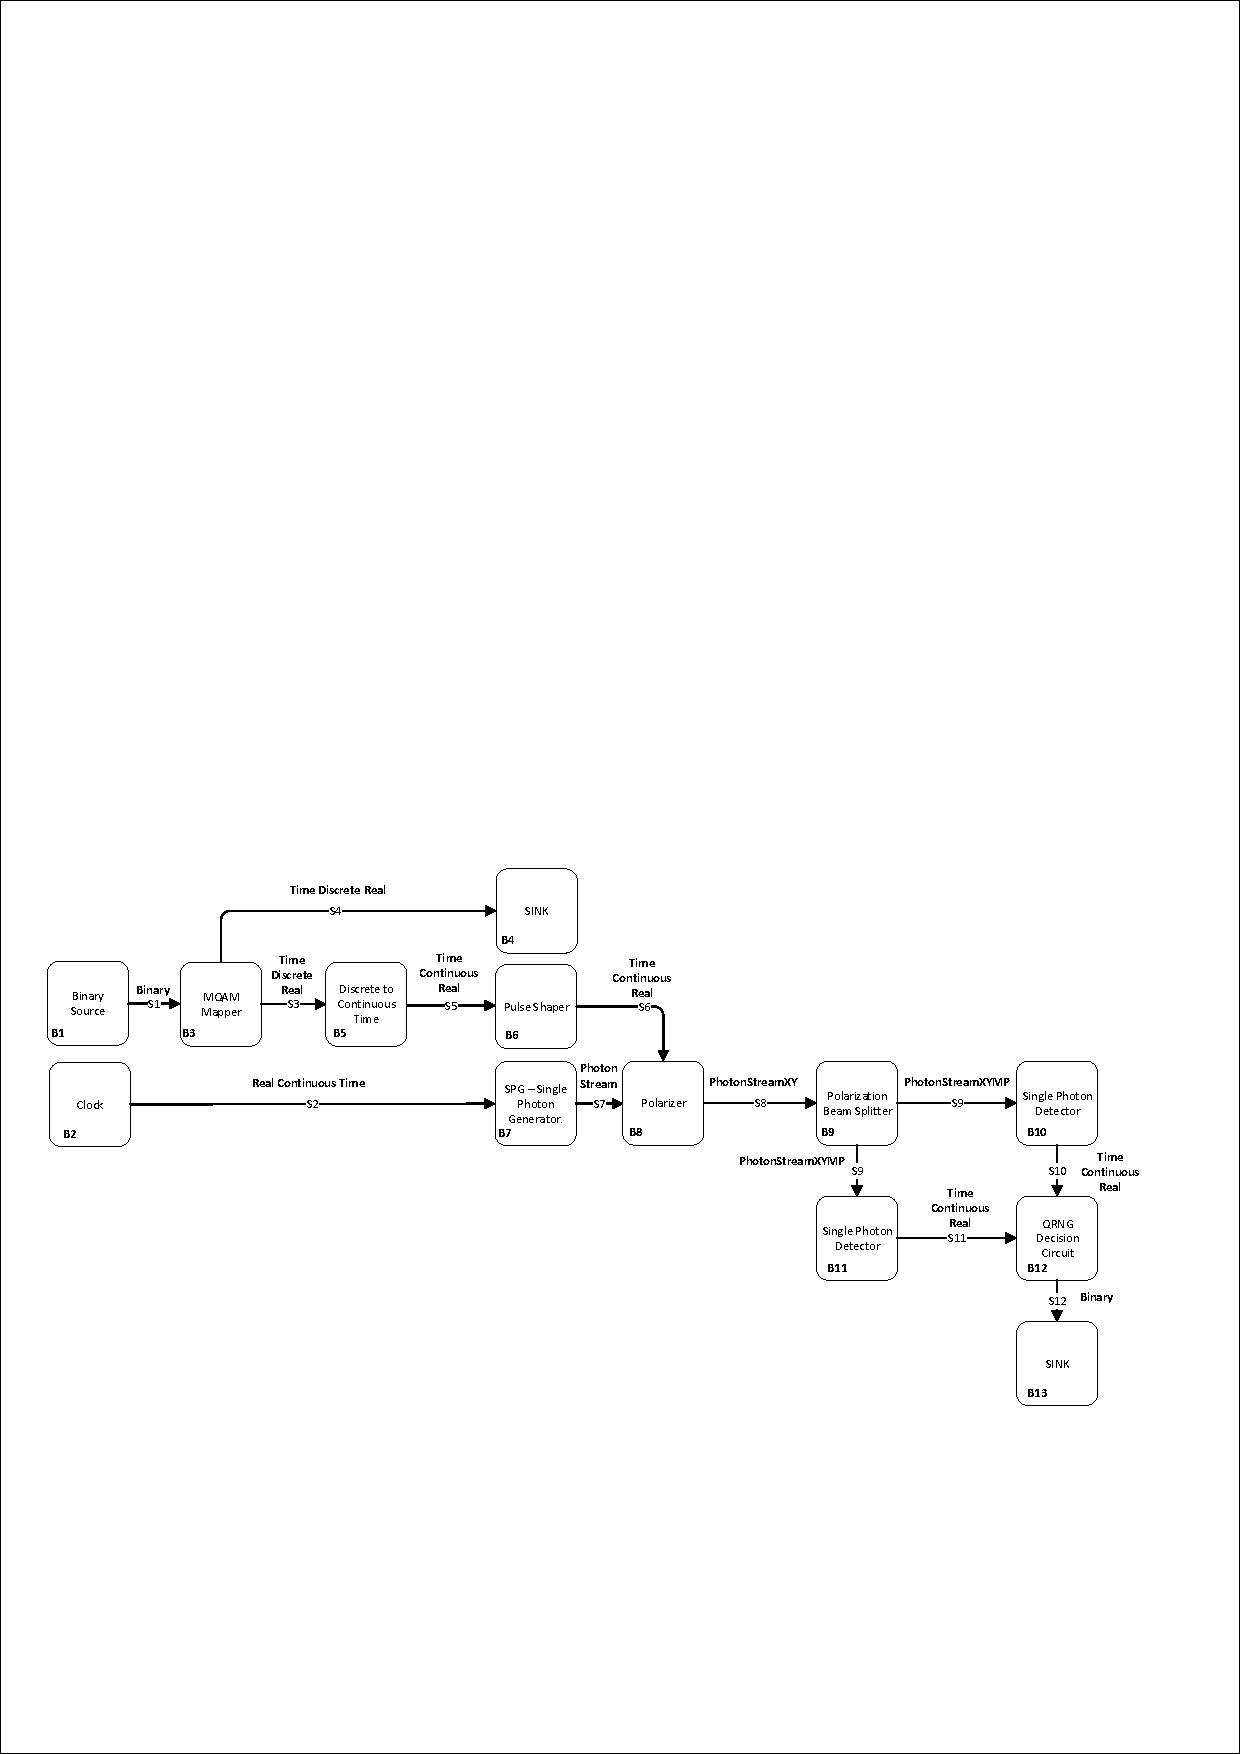
\includegraphics[clip, trim=0.5cm 5cm 0.5cm 14cm, width=1.00\textwidth]{./sdf/quantum_random_number_generator/figures_raw/Simulation_qrng.pdf}
    \caption{Block diagram of the simulation of a Quantum Random Generator.}\label{sim_qrng}
\end{figure}

The simulation diagram of the setup described in the previous section is presented in figure \ref{sim_qrng}. As one can see in the figure, there is a binary source which, in this case, produces a deterministic cycle of binary numbers. The binary stream should be set according to the polarization wished after block Polarizer. Bit stream has two bits, the first bit sets the axis direction and the second bit sets the basis. Table \ref{tb:basisbits} shows the correspondence bits to each basis.

\begin{table}[H]
    \caption{Bits correspondence to each basis.}
     \label{tb:basisbits}
    \centering
    \begin{tabular}{c|c}
    \textbf{\textit{Basis}}         &  \\ \hline
     0 & $+$ \\
     1 & $\times$ \\
    \end{tabular}

\end{table}
Table \ref{tb:rectilinear} shows the correspondent bits for each axis in rectilinear basis.

\begin{table}[H]
    \caption{Bits correspondence of Rectilinear Basis.}
    \label{tb:rectilinear}
    \centering
    \begin{tabular}{c|c}
                & Basis "+" \\ \hline
     0 & $\to (0^{\circ})$ \\
     1 & $\uparrow (90^{\circ})$ \\
    \end{tabular}

\end{table}

Table \ref{tb:diagonal} shows the correspondent bits for each axis in diagonal basis.

\begin{table}[H]
    \caption{Bits correspondence of Diagonal Basis.}
    \label{tb:diagonal}
    \centering
    \begin{tabular}{c|c}
          & Basis "$\times$" \\ \hline
     0 & $\searrow (-45^{\circ})$ \\
     1 & $\nearrow (45^{\circ})$ \\
    \end{tabular}

\end{table}

According with the previous tables, in order to have a polarizer at $45^\circ$, the bit stream in binary source block should be $\{1,1\}$. This way, single photons from source will reach the polarization beam splitter polarized at $45^\circ$ and the photon has $50\%$ of follow the horizontal path or the vertical path. Therefore, each single photon detector has the same probability of detect the photon. However, if one of the detectors flips, the other will not flip.

In addition, the photons are generated by single photon source block at a rate defined by the clock rate.

At the end of the simulation there is a circuit decision block which will outputs a binary signal with value '$0$' if the detector at the end of the horizontal path clicks or '$1$' if the detector at the end of the vertical path clicks.

In table \ref{tb:inputparameters2} are presented the input parameters of the system.


\begin{table}[H]
\centering
\caption{System Input Parameters}
\label{tb:inputparameters2}
\begin{tabular}{|c|c|c|}
\hline
\textbf{Parameter}                      & \textbf{Default Value}                                       \\ \hline
RateOfPhotons                           & 1e6                                                          \\ \hline
NumberOfSamplesPerSymbol                & 16                                                           \\ \hline
vector<t\_iqValues> iqAmplitudeValues   & \{ 0.0,0.0 \},\{ -45.0,0.0 \},\{ 90.0,0.0 \},\{ 45.0,0.0 \}  \\ \hline

\end{tabular}
\end{table}

In table \ref{tb:signals2} are presented the system signals to implement the simulation presented in figure \ref{sim_qrng}.
\begin{table}[H]
\centering
\caption{System Signals}
\label{tb:signals2}
\begin{tabular}{|c|c|c|}
\hline
\textbf{Signal name}                            & \textbf{Signal type}                      \\ \hline
S1                                              &  Binary                                   \\ \hline
S2                                              &  TimeContinuousAmplitudeContinuousReal    \\ \hline
S3                                              &  TimeDiscreteAmplitudeDiscreteReal        \\ \hline
S4                                              &  TimeDiscreteAmplitudeDiscreteReal        \\ \hline
S5                                              &  TimeContinuousAmplitudeDiscreteReal      \\ \hline
S6                                              &  TimeContinuousAmplitudeDiscreteReal      \\ \hline
S7                                              &  PhotonStreamXY                           \\ \hline
S8                                              &  PhotonStreamXY                           \\ \hline
S9                                              &  PhotonStreamXY                           \\ \hline
S10                                             &  TimeContinuousAmplitudeDiscreteReal      \\ \hline
S11                                             &  TimeContinuousAmplitudeDiscreteReal      \\ \hline
S12                                             &  Binary                                   \\ \hline
\end{tabular}
\end{table}

Table \ref{tb:signalsh} presents the header files used to implement the simulation as well as the specific parameters that should be set in each block. Finally, table \ref{tb:signalss} presents the source files.

\begin{table}[H]
\centering
\caption{Header Files}
\label{tb:signalsh}
\begin{tabular}{|c|c|c|}
\hline
\textbf{File name}                              & \textbf{Description}                                                          & \textbf{Status} \\ \hline
netxpto.h                                       &                                                                               &    \checkmark   \\ \hline
binary\_source.h                                &Mode(DeterministicCyclic)                                                      & \checkmark   \\
                                                &BitStream("01")                                                                & \checkmark   \\
                                                &BitPeriod(1/(2*RateOfPhotons))                                                 & \checkmark   \\ \hline
clock\_20171219.h                               &ClockPeriod(1 / RateOfPhotons)                                                 &    \checkmark   \\ \hline
discrete\_to\_continuous\_time.h                &NumberOfSamplesPerSymbol                                                       &    \checkmark   \\ \hline
m\_qam\_mapper.h                                &IqAmplitudes(iqAmplitudeValues)                                                &    \checkmark   \\ \hline
polarization\_beam\_splitter\_20180109.h        &                                                                               &   \checkmark   \\ \hline
polarizer\_20180113.h                           &                                                                               &    \checkmark   \\ \hline
pulse\_shaper\_20180111.h                       &FilterType(Square)                                                             &     \checkmark  \\ \hline
single\_photon\_detector\_20180111.h            &setPath(0), setPath(1)                                                         &    \checkmark   \\ \hline
single\_photon\_source\_20171218.h              &                                                                               &    \checkmark   \\ \hline
sink.h                                          &                                                                               &    \checkmark   \\ \hline
qrng\_decision\_circuit.h                       &                                                                               &    \checkmark   \\ \hline
\end{tabular}
\end{table}

\begin{table}[H]
\centering
\caption{Source Files}
\label{tb:signalss}
\begin{tabular}{|c|c|c|}
\hline
\textbf{File name}                              & \textbf{Description} & \textbf{Status} \\ \hline
netxpto.cpp                                     &                      &    \checkmark   \\ \hline
binary\_source.cpp                              &                      &    \checkmark   \\ \hline
clock\_20171219.cpp                             &                      &    \checkmark   \\ \hline
discrete\_to\_continuous\_time.cpp              &                      &    \checkmark   \\ \hline
m\_qam\_mapper.cpp                              &                      &    \checkmark   \\ \hline
polarization\_beam\_splitter\_20180109.cpp      &                      &   \checkmark   \\ \hline
polarizer\_20180113.cpp                         &                      &    \checkmark   \\ \hline
pulse\_shaper\_20180111.cpp                     &                      &     \checkmark  \\ \hline
single\_photon\_detector\_20180111.cpp          &                      &    \checkmark   \\ \hline
single\_photon\_source\_20171218.cpp            &                      &    \checkmark   \\ \hline
sink.cpp                                        &                      &    \checkmark   \\ \hline
qrng\_decision\_circuit.cpp                     &                      &    \checkmark   \\ \hline
qrng\_sdf.cpp                                   &                      &    \checkmark   \\ \hline
\end{tabular}
\end{table}

\subsection{Open Issues}


\newpage
\bibliographystyle{unsrt}

\bibliography{bibliography}

\cleardoublepage
